\chapter{Concept}
In this chapter the desired concept will be presented. 

Typical concept: \cite{payan2012soft}
\section{System}
The hardware used with this system consists of:
\begin{itemize}
  \item a tracked ultrasound device
  \item a tracked pointer tool
  \item an optical tracking camera to track the instruments
  \item a computer to run the software
  \item a 3D-monitor which displays the 3D contents of the software 
  \item a touch-screen on a 2D-monitor to operate the software and show the
    ultrasound images
\end{itemize}
The software in this system consists of:
\begin{itemize}
  \item a sampling method 
  \item a reconstruction method 
  \item a segmentation method 
  \item a planning method 
  \item a navigation 
\end{itemize}

\begin{figure}[H]
  \centering
  \begin{tabular}[H]{c c c c c c}
    \multicolumn{2}{c}{\thead{Sampling method \\ to collect points on \\ the liver-surface}} & \multicolumn{2}{c}{\thead{Reconstruction method \\ to reconstruct the surface \\ from the sampled points}} & \multicolumn{2}{c}{\thead{Segmentation method \\ to segment the tumors on \\ the ultrasound images}}
    \\
    \multicolumn{2}{c}{\addheight{
\includegraphics[width=0.3\linewidth]{samplingMethod}}} &
    \multicolumn{2}{c}{\addheight{
\includegraphics[width=0.3\linewidth]{reconstructionMethod}}} &
    \multicolumn{2}{c}{\addheight{
\includegraphics[width=0.3\linewidth]{segmentationMethod}}} 
    \\
    \\
    \\
    \multicolumn{3}{c}{\thead{Planning method \\ to plan the resection \\ of the liver}} & \multicolumn{3}{c}{\thead{Navigation mode used \\ to navigate during the \\ removal of the tumor}} 
    \\
    \multicolumn{3}{c}{\centering \addheight{
\includegraphics[width=0.48\linewidth]{planningMethod}}} &
    \multicolumn{3}{c}{\addheight{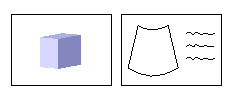
\includegraphics[width=0.48\linewidth]{navigationMode}}} 
    \\
    & & & & &
    % \addheight{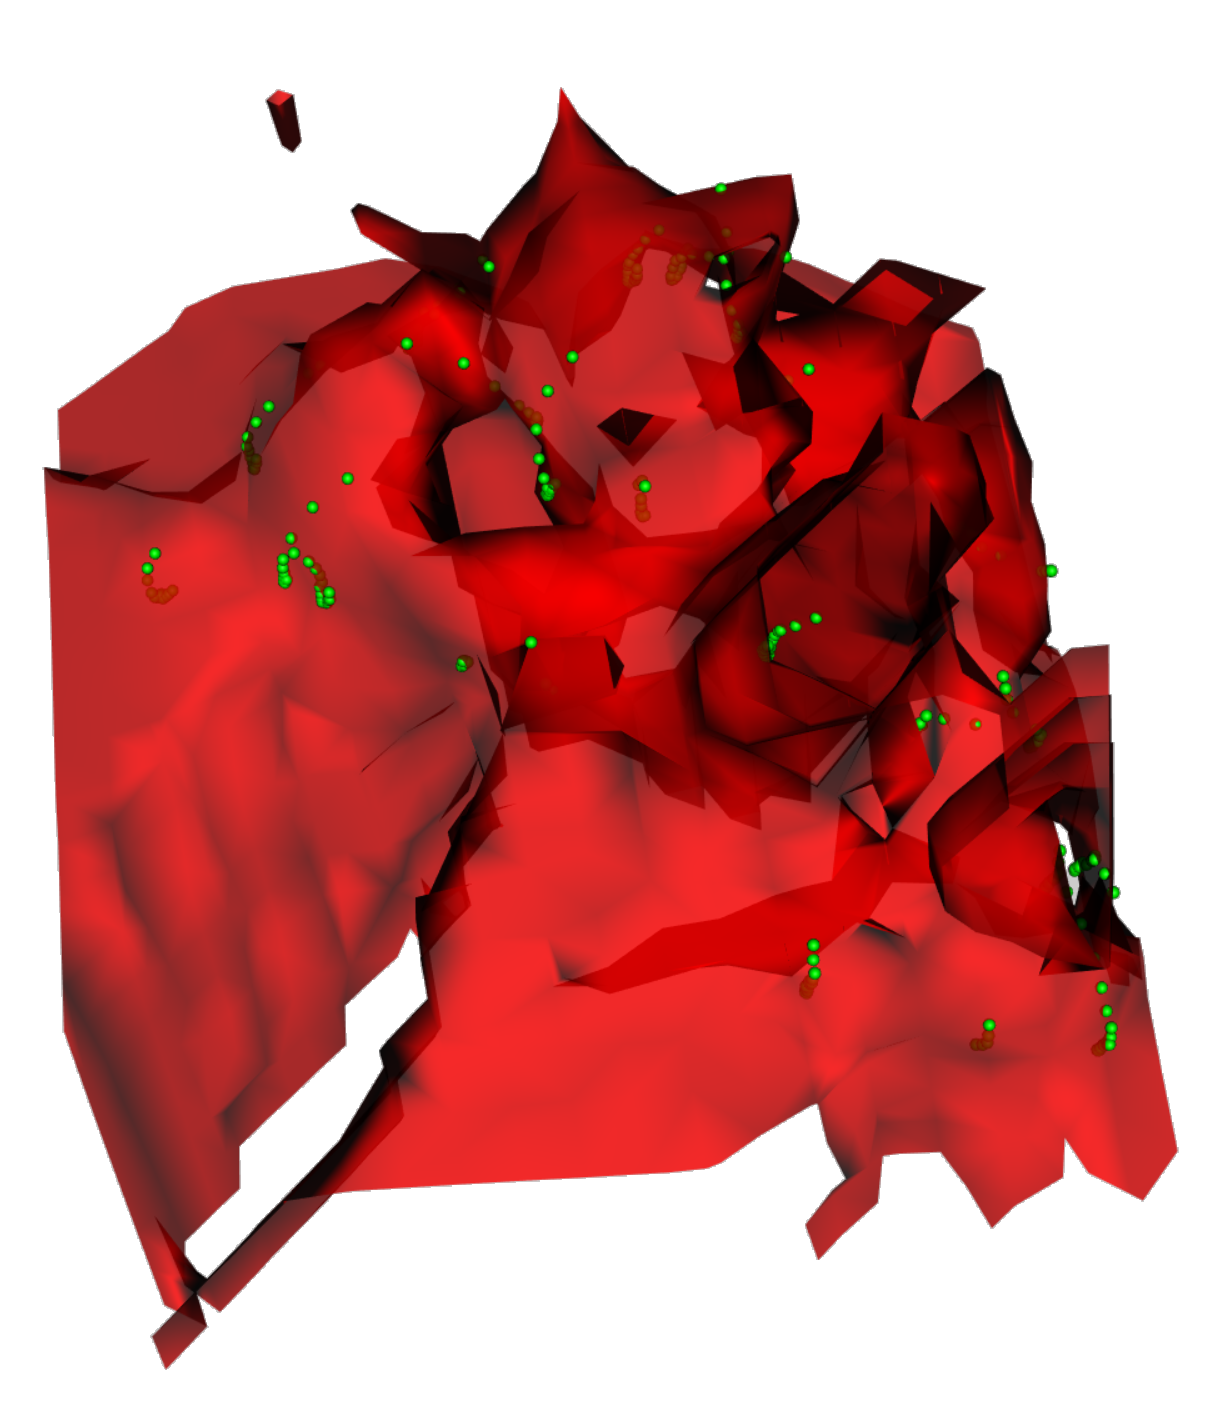
\includegraphics[width=0.3\linewidth]{mes08_pointgrid.png}}
    \\
  \end{tabular}
  \caption{Software components}
  \label{fig:softwareComponents}
\end{figure}
\section{Functionalities}
The three main functionalities of the developed concept will be presented in
this chapter. These functionalities were specifically developed for this project.
\subsection{Surface Reconstruction}
During surgery ultrasound images and their corresponding 6D poses (positions and
orientations) are collected and analyzed. First each ultrasound image has to be
checked for contact with the liver. If the ultrasound passes the check, that
means the ultrasound image looks like an ultrasound image that can only arise
when the ultrasound probe lies on the liver surface, then the position of this
image can be used.

\begin{figure}[H]
  \centering
  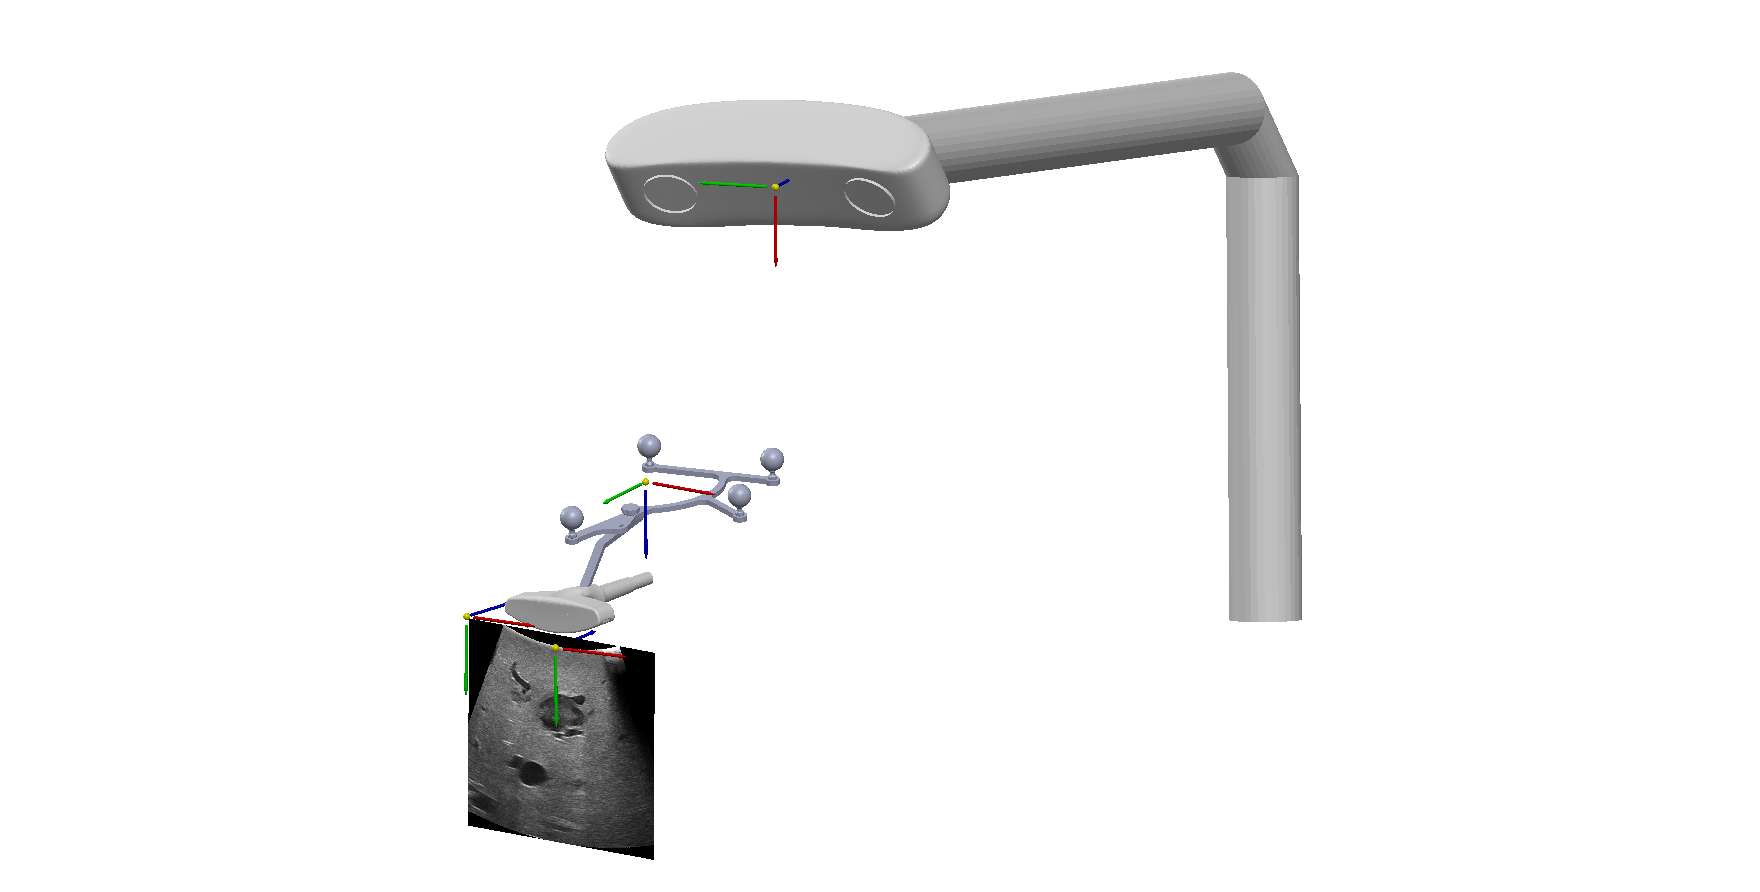
\includegraphics[width=1.0\textwidth]{Assembly}
  \caption{The different coordinate systems}
  \label{fig:Assembly}
\end{figure}

\textcolor{red}{In order to use ... too complicated. Put an image for that and name the transformations.}
In order to use the sampled position corresponding to an image, this
position has to be transformed into the correct coordinate system first. There
are four different coordinate systems. The first coordinate system is the image
coordinate system. The units in the image coordinate system are pixels and the
origin is in the top left corner of the image. The
second coordinate system is the ultrasound coordinate system. The origin of this
coordinate system is at the probe tip in the middle and the units in this and
the following coordinate systems are millimeters. The third coordinate system is the
ultrasound-tool-marker coordinate system. The origin is at a user defined
location, relative to the reflective marker spheres. The final
coordinate system is the tracking camera coordinate system. The origin of this
coordinate system is at the position sensor in the tracking camera and can not
be changed.

At the end of this transformation chain, a image pixel 2D position was
transformed into a tracking camera 3D positon and the units changed
from pixel to millimeter. This 3D location in the tracking camera coordinate system
will be added to the collection of points to later reconstruct the surface from.

After collecting the surface points, the reconstruction algorithm from Hoppe
\cite{hoppe1992surface} reconstructs the surface from these points.
\subsection{Tumor Segmentation}
To reconstruct and later plan the resection of a tumor, the shape
of the tumor has to be made visible first. Because most liver tumors are not visible from the outside of the liver, an
ultrasound device is often used during liver resections to look behind the
liver surface.

Therefore this ultrasound device should also be used to
reconstruct the shape of a tumor. This is done by segmenting the same tumor on
multiple ultrasound images. Depending on the desired resolution of the
reconstructed tumor, more or less images have to be segmented. With the corresponding
poses of the ultrasound images, the 3D positions of the individual contour
pixels can be calculated. These positions will create a point cloud that
represents the shape of the tumor. This shape can then be reconstructed by a
surface reconstruction algorithm.
\subsubsection{Semi automatic 3D}
In order to semi automatically segment a tumor in the liver, the segmentation
has to be initialized manually. To do so, a sphere needs to be
placed in the center of the tumor manually. Afterwards each ultrasound image
which cuts this sphere will be segmented automatically with the cutted area as
an initialization for the segmentation. These segmentations would be used to
reconstruct the surface of the tumor.
\subsection{Resection Planning}
For parenchymal-sparing liver resections, the goal is to keep as much healthy tissue as
possible. When the tumor's location in the liver and the size are known, one can plan a
precise resection from these informations. The surgeon is able to choose
which shape the resection plane will have and how much safety margin he wants to
add around the tumor. Then a resection plane which fulfills the desired requirements
will be shown to the surgeon. This resection plane could then be fine tuned before the
surgeon starts the resection.
% After collecting the needed
% information as described in the previous sections, the planning can 

\section{Workflow}
In this section the conceptual workfolw through a liver resection using the
desired system will be presented. The following flow diagram shows the five main
steps (Figure \ref{fig:conceptWorkflow}).
\begin{figure}[H]
  \centering
  \smartdiagram[sequence diagram]{Preparation, Liver scanning, Tumor scanning,
    Resection planning,  Removal of the tumor}
  \caption{The main steps the surgeon has to do during a surgery with the
    proposed system.}
  \label{fig:conceptWorkflow}
\end{figure}
In the preparation step the patient is prepared for the surgery, the
navigation system is setup in the operating room and the software is started.
Then the tools are setup. Afterwards the surgery starts, the intervention starts and the liver gets
prepared for the resection. Subsequently step two starts. In this step the
surgeon scans the liver surface with an ultrasound probe. He does that till a 3D
model of the for the surgery needed part of liver is reconstructed. Thereafter
follows the tumor scanning step. Here the surgeon locates a tumor using the
ultrasound probe again. Then he freezes the ultrasound image and initializes the
segmentation of it. After this the surgeon moves the ultrasound probe in
different directions such that the ultrasound images cut through the tumor. He
does that till the tumor is accurately enough reconstructed. Afterwards follows
step four. To plan the resection the surgeon has to select the shape of the
resection plane he wants to apply for this resection intervention. If necessary
he adjusts the resection plane manually. Finally he uses the created model and
planning to resect the tumor. 
% By use of the initialization the tumor is
% segmented on the ultrasound images. Then the segmentations are combined in order
% to reconstruct a 3D model of the tumor.  
\subsection{Resection planning for non-anatomical ...}

%%% Local Variables:
%%% TeX-master: "MscThesis"
%%% End: